\documentclass[../main.tex]{subfiles}
\graphicspath{{\subfix{../images/}}}
\begin{document}

\subsection{Related Work}
Longman et. al. \cite{longman_multipath_2021} introduced a method for multipath mitigation under the above assumptions which they applied to vehicles. Their goal was to estimate the reflection surface between all candidate real-ghost pairs and classify candidates using a correlation criteria.
fig~\ref{fig:method} provides a high level illustration of the method. Given a pair of tracks with a single point each, the reflection line is given by:
\begin{equation}
    y = tan(\alpha) x + b
\end{equation}

and the ghost line, i.e the line from the ego-vehicle to the ghost target is given by:
\begin{equation}
    y = tan(\beta) x
\end{equation}

\par
The algorithm is detailed in Alg.\ref{alg:orig}. Given a set of candidate track pairs, one can estimate a set of points on the reflection surface by assosiation of points from both clusters and measuring the intersection of the reflection line and the ghost line. Once such set of points has been obtained, a line is fitted to it using linear regression allowing for correlation criteria to be calculated:
\begin{itemize}
    \item MSD: This criteria measures the linearity of the estimated reflection surface.
    \item ANG: This criteria measures the alignment between the estimated surface angle and the fitted linear line angle.
\end{itemize}

\par
A low result for both criteria means that the estimated refleciton surface has low fitting error, implying that the candidate tracks fit the rea-ghost model and that one is indeed a refleciton of the other. Following the multipath model described above, the ghost target will always be the one with larger range to the ego-vehicle.


\begin{algorithm}
\caption{Longman et. al. Multipath Mitigation}\label{alg:orig}
\begin{algorithmic}

\State $C = \{(t_{r1},t_{g1}), ..., (t_{rn},t_{gn})\}$  real-ghost candidates\;

\State \# Estimate reflection surface points
\For{$(t_r,t_g) \in C$}
    \For{$(x_r, y_r) \in t_r, (x_g, y_g) \in t_g$}
        \State $m \gets \frac{y_t-y_g}{x_t-x_g}$
        \State $a \gets tan^{-1}(m)-\frac{\pi}{2}$
        \State $b \gets \frac{y_t+y_g}{2}-tan(a)\frac{x_t+x_g}{2}$
        \State $\beta \gets tan^{-1}(y_g/x_g)$
        \State $x_r \gets \frac{b}{\tan(\beta) - \tan(a)}$
        \State $y_r \gets \tan(\beta)x_r$
        \State $r \gets (x_r, y_r)$
    \EndFor\;\\
    $l_r \gets (\Vec{x_r}, \Vec{y_r})$ \;
\EndFor\;\\

\State \# Fit a line to reflection points
\State $\hat{l_r} \gets linreg(\{r_1, r_2, ... , r_n\}) = (\Vec{\hat{x_r}}, \Vec{\hat{y_r}})$\;\\

\State \# Calculate correlation criteria
\State $MSD \gets E[(\Vec{x_r}-\Vec{\hat{x_r}})^2 + (\Vec{y_r}-\Vec{\hat{y_r}})^2]$\;
\State $ANG \gets E[\vec{a}-\tan^{-1}{(\frac{\Vec{\hat{y_r}}}{\Vec{\hat{x_r}}})}]$\;
\end{algorithmic}
\end{algorithm}

\begin{figure}[htbp]
    \centerline{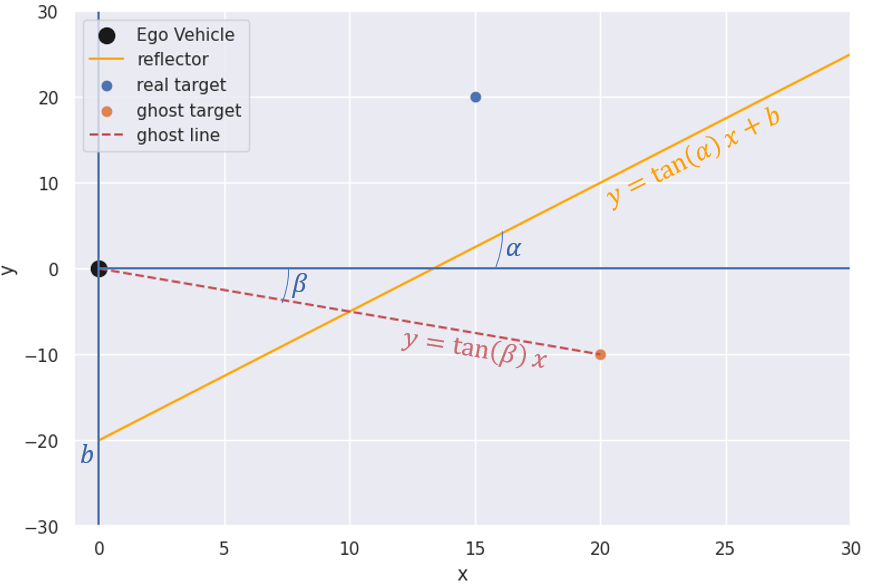
\includegraphics[scale=0.33]{figures/fig_method.png}}
    \caption{Illustration of multipath scenario. The estimated line parameters are obtained by geometric calculations given a point from each target candidate. Using the estimated ghost line and reflector line, the intersection point is obtained.}
    \label{fig:method}
\end{figure}

This method was applied to vehicles, which tend to spread across several range-azimuth bins in radar detections and have a relatively strong SNR due to their large metallic body.

\subsection*{VRUs Multipath Mitigation}
In order to apply  the method to VRUs, some adjustments are needed to compensate for the smaller size and weaker signal of such targets. Smaller targets lead to clusters with less detections and less spatial spread compared to vehicles. The purposed solution for this issue is to aggregate the radar detections across multiple timestamps. 
This effectively increases the number of points per cluster, and since the objects are dynamic, it also increases the spatial spread of the points. This is important since robust estimation of the reflection surface requires large and diverse clusters.
Fig.~\ref{fig:agg} illustrates how aggregating radar frames effectively increases the number of points in each dynamic track.

\par
Aggregating the radar frames is a delicate tradeoff between improving performance and increasing algorithm latency. Since automotive radar requires minimal procssing time, aggerating was capped at a maximum of 3 consecutive frames.\\

\par
Applying the multipath mitigation method to real-world data requires handling candidate cluster pairs where one cluster is larger than the other. This may be caused by indirect return signals with attenuated amplitude that were not detected, or simply due to the fact that the indirect path does not cover the entire object while the direct path does. 
For the scope of this work, the estimated number of point was determined by the size of the smaller cluster and point assosiation was done by sorting each cluster by range.

\begin{figure}[htbp]
% \centerline{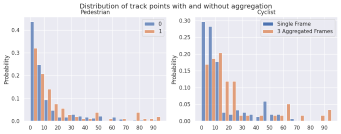
\includegraphics{figures/fig_aggregation2_small.png}}
\centerline{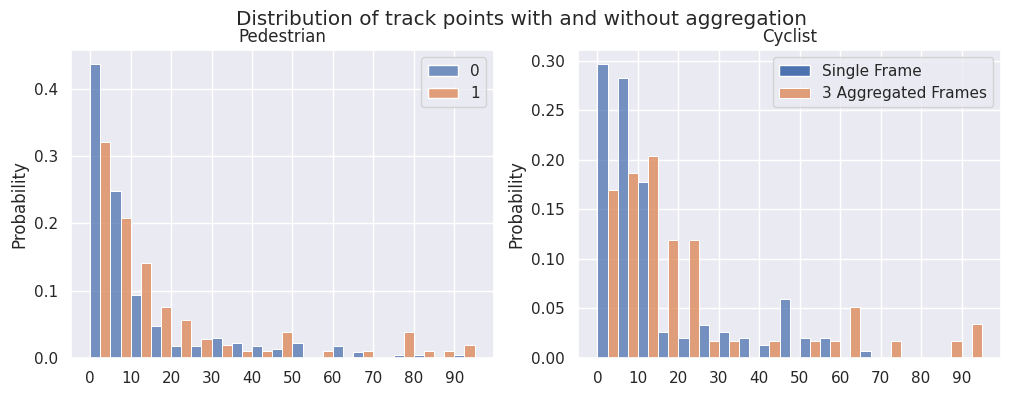
\includegraphics[scale=0.33]{figures/fig_aggregation2.png}}
\caption{Distribution of number of points per dynamic track with and without aggregation. Both sub-figures depict the same scene - outgoing VRU. Left: Pedestrian, Right: Cyclist}
\label{fig:agg}
\end{figure}


\end{document}